\subsection{Código Bloque \textit{Acensor}:} \label{code:Acensor}

\subsection{Código Bloque \textit{Acensor (testbench)}:} \label{code:Acensor_tb}

\subsection{Código Bloque \textit{Controlador Motor}:} \label{code:ControladorMotor}

\subsection{Código Bloque \textit{Controlador Motor (testbench)}:} \label{code:ControladorMotor_tb}

\subsection{Código Bloque \textit{Controlador Puerta}:} \label{code:ControladorPuerta}

\subsection{Código Bloque \textit{Controlador Puerta (testbench)}:} \label{code:ControladorPuerta_tb}

\subsection{Código Bloque \textit{Decodificador a 7 segmentos}:} \label{code:Decodificador7s}
	\inputminted[frame=lines,fontsize=\footnotesize,linenos]{vhdl}{CodeFiles/Decodificador7s.vhd}

\subsection{Código Bloque \textit{Decodificador a 7 segmentos (testbench)}:} \label{code:Decodificador7s_tb}
	Utilizando este testbench se obtiene el comportamiento que se puede ver en la Figura (\ref{fig:SimulacionDecodificador7s}):

    \begin{figure}[H]
		    \centering
		    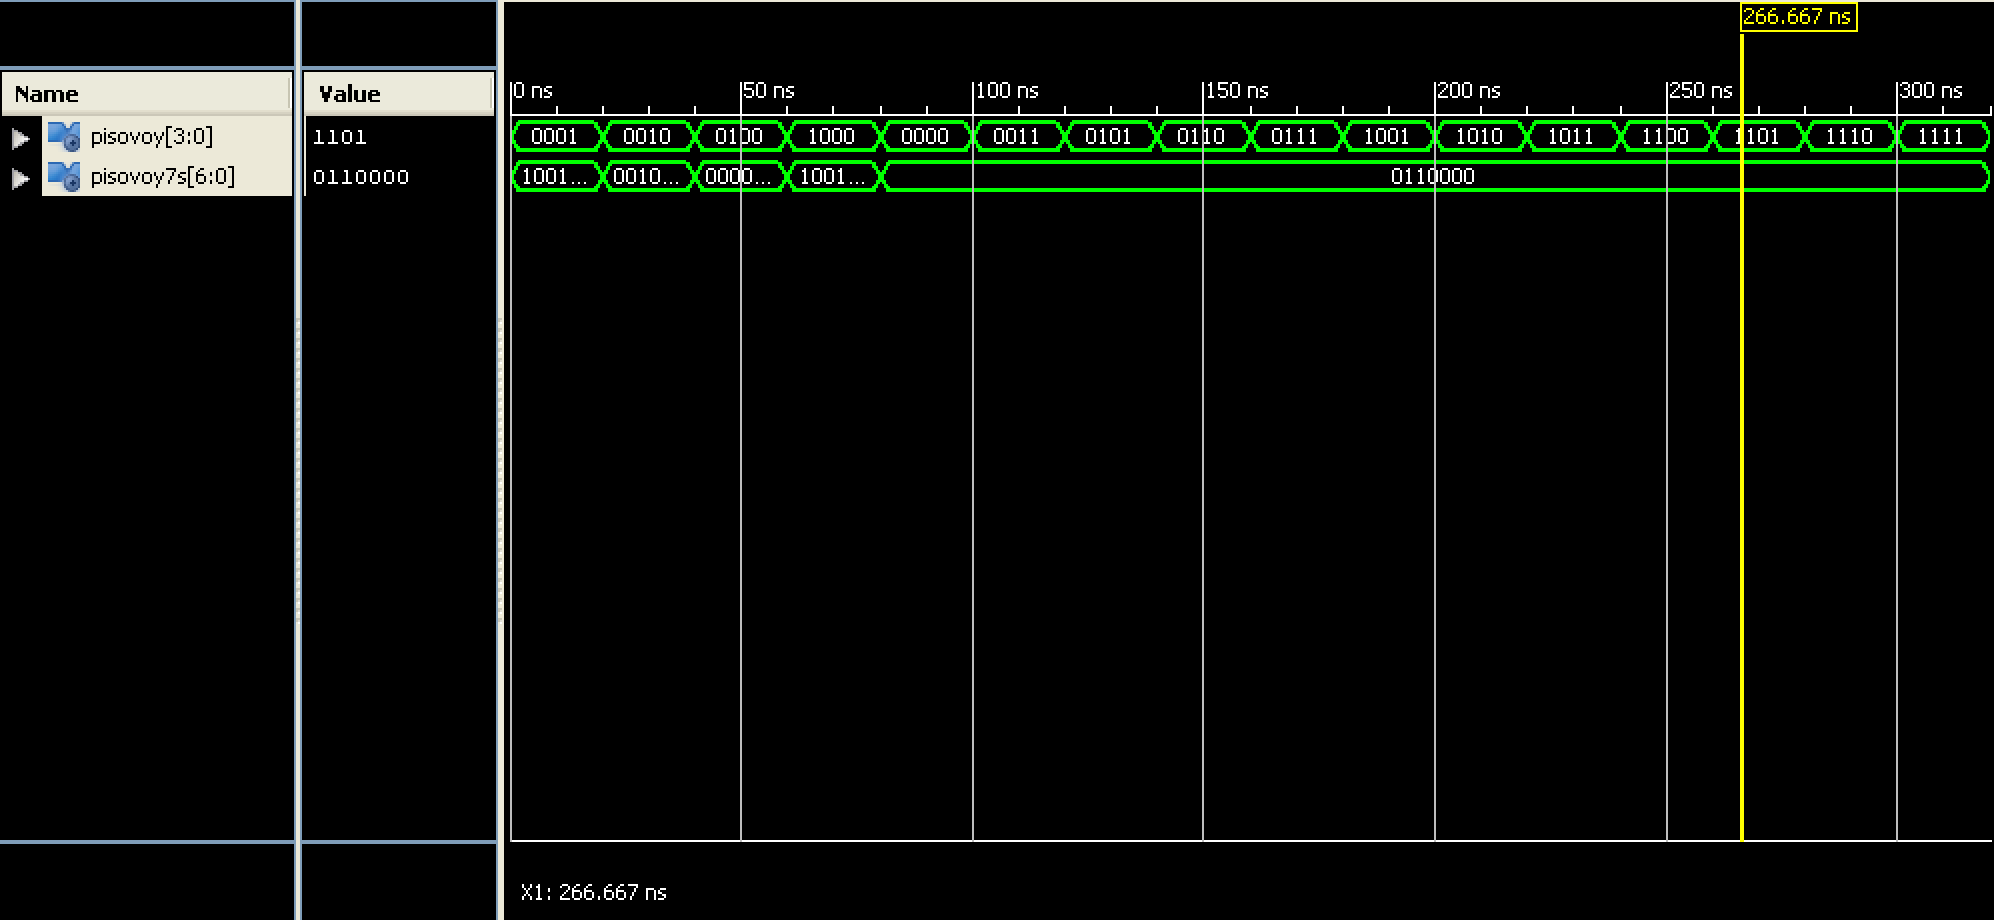
\includegraphics[width = 0.8\textwidth ]{SimulacionDecodificador7s}
		    \caption{Simulación del testbench del bloque Decodificador7s}
		    \label{fig:SimulacionDecodificador7s}
	\end{figure}
	\inputminted[frame=lines,fontsize=\footnotesize,linenos]{vhdl}{CodeFiles/Decodificador7s_tb.vhd}

\subsection{Código Bloque \textit{Divisor de frecuencia}:} \label{code:DivisorFrecuencia}

\subsection{Código Bloque \textit{Divisor de frecuencia (testbench)}:} \label{code:DivisorFrecuencia_Tb}

\subsection{Código Bloque \textit{PistoActual}:} \label{code:PisoActual}
    \inputminted[frame=lines,fontsize=\footnotesize,linenos]{vhdl}{CodeFiles/PisoActual.vhd}
    
\subsection{Código Bloque \textit{PistoActual (testbench)}:} \label{code:PisoActual_tb}
    \inputminted[frame=lines,fontsize=\footnotesize,linenos]{vhdl}{CodeFiles/PisoActual_tb.vhd}
    
\subsection{Código Bloque \textit{Comportamiento Interno}:} \label{code:ComportamientoInterno}

\subsection{Código Bloque \textit{Comportamiento Interno (testbench)}:} \label{code:ComportamientoInterno_tb}

\subsection{Código Bloque \textit{Bloqueador pisoVoy}:} \label{code:BloqueadorpisoVoy}	
    \inputminted[frame=lines,fontsize=\footnotesize,linenos]{vhdl}{CodeFiles/BloqueadorpisoVoy.vhd}

\subsection{Código Bloque \textit{Bloqueador pisoVoy (testbench)}:} \label{code:BloqueadorpisoVoy_tb}
    \inputminted[frame=lines,fontsize=\footnotesize,linenos]{vhdl}{CodeFiles/BloqueadorpisoVoy_tb.vhd}

    Utilizando este testbench se obtiene el comportamiento que se puede ver en la Figura (\ref{fig:SimulacionBloqueadorPisoVoy}):

    \begin{figure}[H]
		    \centering
		    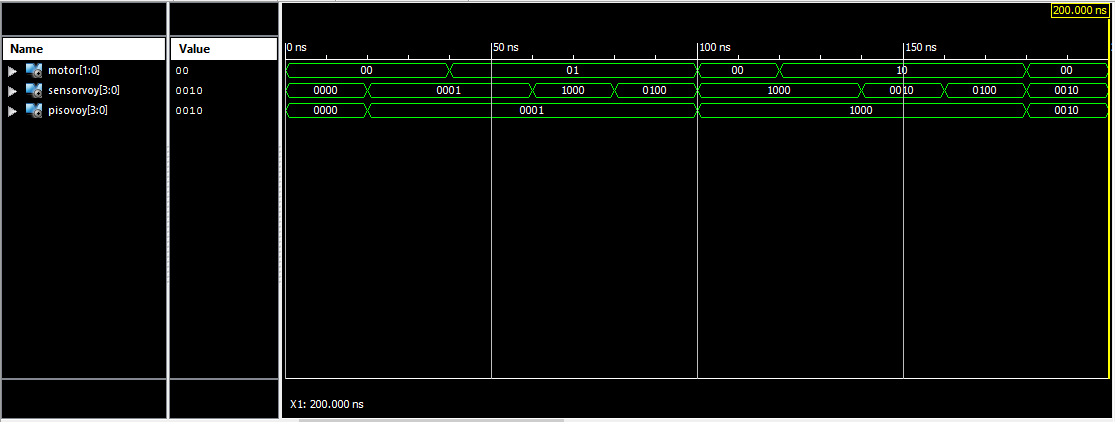
\includegraphics[width = 0.8\textwidth ]{SimulacionBloqueadorPisoVoy}
		    \caption{Simulación del testbench del bloque BloqueadorPisoVoy}
		    \label{fig:SimulacionBloqueadorPisoVoy}
	\end{figure}

\subsection{Código Bloque \textit{Decodificador Binario a Decimal}:} \label{code:DecodificadorBinarioDecimal}
    \inputminted[frame=lines,fontsize=\footnotesize,linenos]{vhdl}{CodeFiles/DecodificadorBinarioDecimal.vhd}
    
    Como se puede ver en la Figura (\ref{fig:BloqueDecodificadorBinarioDecimalOK}) el esquema obtenido una vez programado y sintetizado se corresponde con el quepretendía.
    \begin{figure}[H]
		    \centering
		    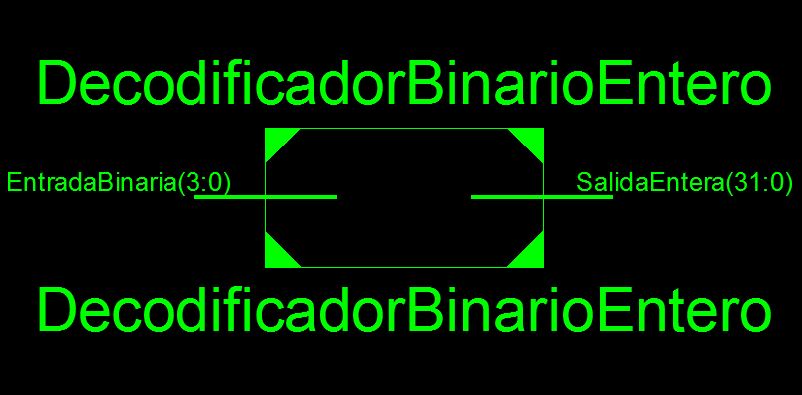
\includegraphics[width = 0.8\textwidth ]{BloqueDecodificadorBinarioDecimalOK}
		    \caption{Salida en los displays de 7 segmentos}
		    \label{fig:BloqueDecodificadorBinarioDecimalOK}
	\end{figure}
    Además podemos ver en la Figura (\ref{fig:BloqueDecodificadorBinarioDecimalImplementacion}) como se compone internamente el bloque, como se codifica en hardware esta utilidad:
    \begin{figure}[H]
		    \centering
		    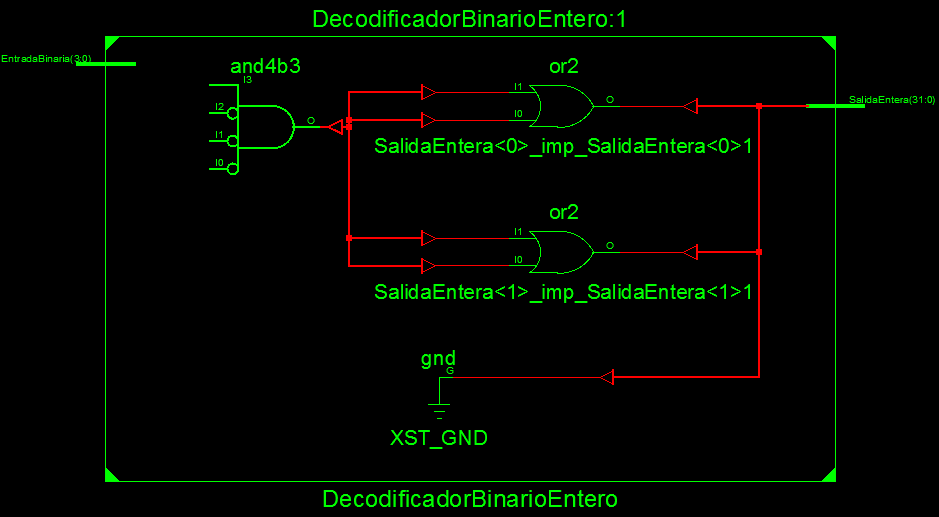
\includegraphics[width = 0.8\textwidth ]{BloqueDecodificadorBinarioDecimalImplementacion}
		    \caption{Salida en los displays de 7 segmentos}
		    \label{fig:BloqueDecodificadorBinarioDecimalImplementacion}
	\end{figure}
    
\subsection{Código Bloque \textit{Decodificador Binario a Decimal (testbench)}:} \label{code:DecodificadorBinarioDecimal_tb}
    \inputminted[frame=lines,fontsize=\footnotesize,linenos]{vhdl}{CodeFiles/DecodificadorBinarioDecimal_tb.vhd}
    
\subsection{Código Bloque \textit{Comparador}:} \label{code:Comparador}
    \inputminted[frame=lines,fontsize=\footnotesize,linenos]{vhdl}{CodeFiles/Comparador.vhd}	

\subsection{Código Bloque \textit{Comparador (testbench)}:} \label{code:Comparador_tb}
